%\begin{frame}
%  \frametitle{Sparse Grids -- Basics}
%  \topline
%  \vspace{-10px}
%  \begin{block}{Hierarchical Basis}
%    \begin{figure}[!htp]
%      \setbeamertemplate{caption}{\raggedright\insertcaption\par}
%      \setbeamerfont{caption}{size=\footnotesize}
%      \centering
%      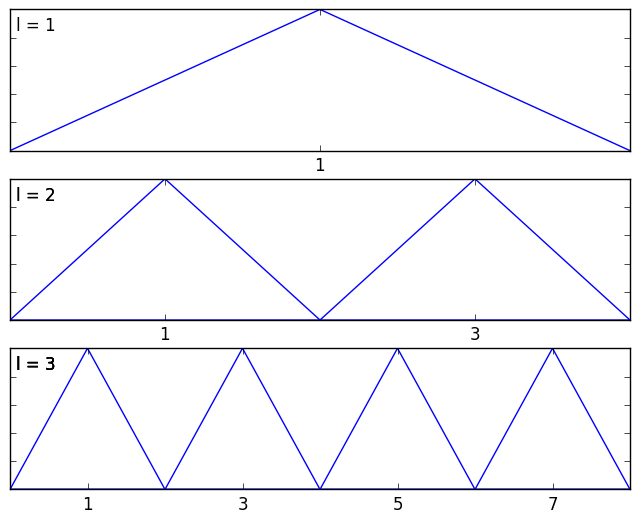
\includegraphics[width=7.5cm]{images/sparse_hats}
%      \vspace{-12px}
%      \caption{}
%    \end{figure}
%  \end{block}
%\end{frame}

\begin{frame}
  \frametitle{Sparse Grids -- Basics}
  \topline
  \vspace{-10px}
  \begin{block}{Hierarchical vs. nodal basis}
    \begin{figure}[!htp]
      \setbeamertemplate{caption}{\raggedright\insertcaption\par}
      \setbeamerfont{caption}{size=\footnotesize}
      \centering
      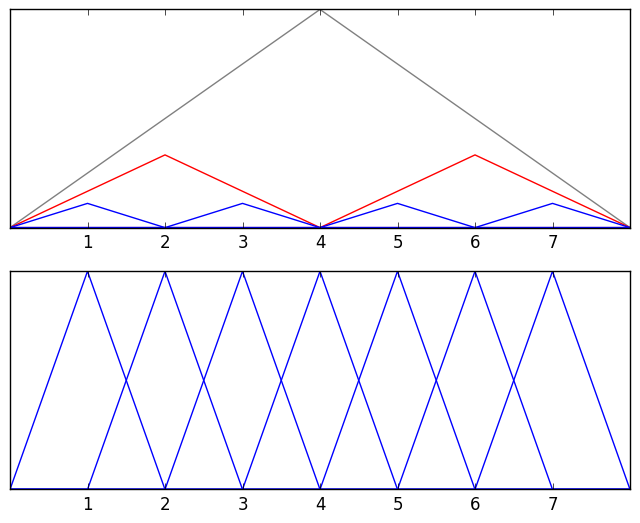
\includegraphics[width=7.5cm]{images/sparse_together}
      \vspace{-12px}
      \caption{}
    \end{figure}
  \end{block}
\end{frame}

\begin{frame}
  \frametitle{Sparse Grids -- Basics}
  \topline
  \vspace{-10px}
  \begin{block}{Hierarchical basis}
    \begin{itemize}
      \item Grouping grid points into levels $l \in \{1,2,3\dots , n\}$
      \item Basis function by index \textbf{and} level: $\phi_{l,i}(x)$
    \end{itemize}
    \vspace{20px}
      $$\hat{f}(x) = \sum_{l \leq n,i \in G_l}{\ \alpha_{l,i} \cdot \phi_{l,i}(x)}$$
  \end{block}
\end{frame}


\begin{frame}
  \frametitle{Sparse Grids -- Basics}
  \topline
  \vspace{-10px}
  \begin{block}{Hierarchical Basis}
    \begin{figure}[!htp]
      \setbeamertemplate{caption}{\raggedright\insertcaption\par}
      \setbeamerfont{caption}{size=\footnotesize}
      \centering
      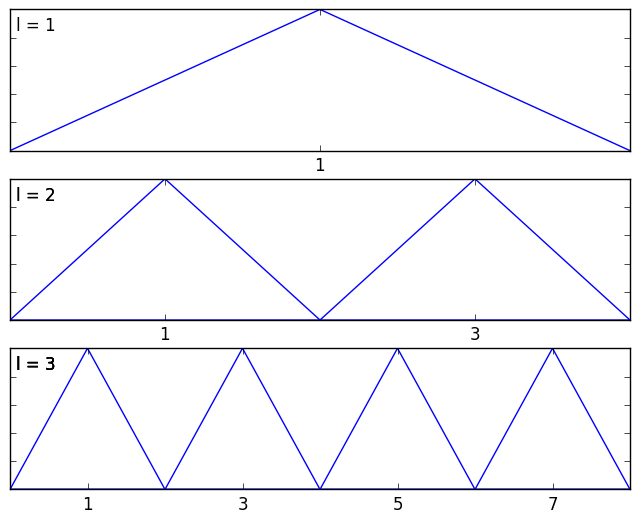
\includegraphics[width=7.5cm]{images/sparse_hats}
      \vspace{-12px}
      \caption{}
    \end{figure}
  \end{block}
\end{frame}

\begin{frame}
  \frametitle{Sparse Grids -- Basics}
  \topline
  \vspace{-10px}
  \begin{block}{Discretization with hierarchical basis}
    \begin{figure}[!htp]
      \setbeamertemplate{caption}{\raggedright\insertcaption\par}
      \setbeamerfont{caption}{size=\footnotesize}
      \centering
      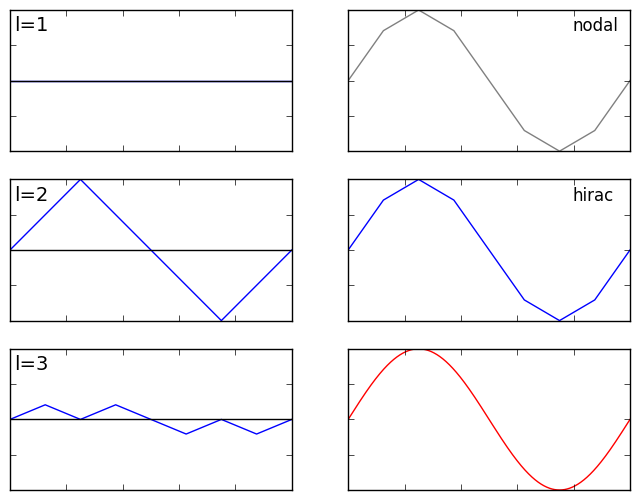
\includegraphics[width=7.5cm]{images/sparsegrid_1d_1}
      \vspace{-12px}
      \caption{}
    \end{figure}
  \end{block}
\end{frame}


\begin{frame}
  \frametitle{Sparse Grids -- Basics}
  \topline
  \vspace{-10px}
  \begin{block}{Discretization with hierarchical basis}
    \begin{figure}[!htp]
      \setbeamertemplate{caption}{\raggedright\insertcaption\par}
      \setbeamerfont{caption}{size=\footnotesize}
      \centering
      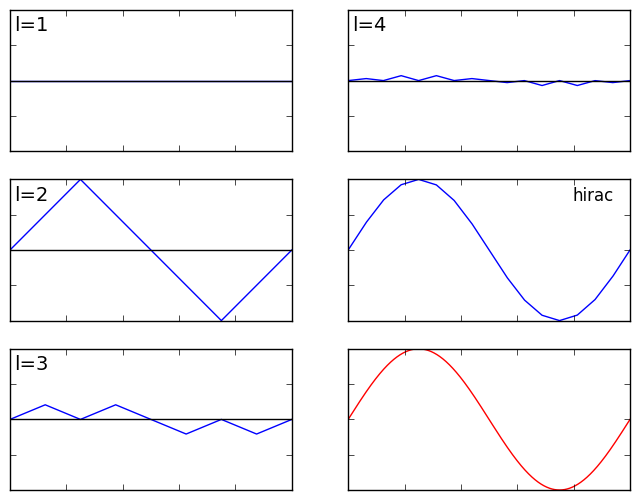
\includegraphics[width=7.5cm]{images/sparsegrid_1d_2}
      \vspace{-12px}
      \caption{}
    \end{figure}
  \end{block}
\end{frame}

\begin{frame}
  \frametitle{Sparse Grids -- Basics}
  \topline
  \vspace{-10px}
  \begin{block}{Hierarchical basis for $d > 1$}
    \begin{itemize}
      \item Index and level vector $\vec{i}$, $\vec{l}$
      \item Combination of levels in all dimensions
      \item Notion of subspaces
    \end{itemize}
  \end{block}
\end{frame}

\begin{frame}
  \frametitle{Sparse Grids -- Basics}
  \topline
  \vspace{-10px}
  \begin{block}{Hierarchical basis: Grid points}
    \begin{figure}[!htp]
      \setbeamertemplate{caption}{\raggedright\insertcaption\par}
      \setbeamerfont{caption}{size=\footnotesize}
      \centering
      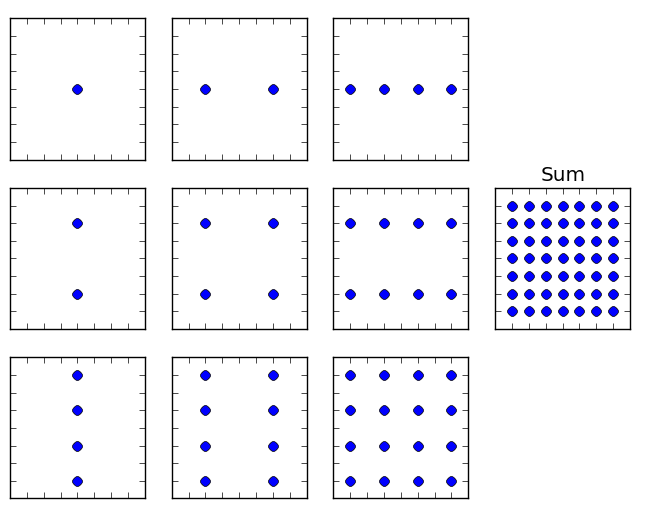
\includegraphics[width=7.5cm]{images/sparsegrid_hirach1}
      \vspace{-12px}
      \caption{}
    \end{figure}
  \end{block}
\end{frame}
\begin{frame}
  \frametitle{Sparse Grids -- Basics}
  \topline
  \vspace{-10px}
  \begin{block}{Sparse grid -- Changes}
    \begin{itemize}
      \item Certain subspaces get disregarded
      \item Finding those is a \emph{a-priori} solvable optimization problem
      \item The resulting grid is \textbf{sparse}
      \end{itemize}
  \end{block}
  \begin{block}{Profit}
    \begin{itemize}
      \item Reducing the computational effort ``a lot''
      \item Maintaining ``high'' accuracy
      \end{itemize}
  \end{block}
\end{frame}

\begin{frame}
  \frametitle{Sparse Grids -- Basics}
  \topline
  \vspace{-10px}
  \begin{block}{A sparse grid}
    \begin{figure}[!htp]
      \setbeamertemplate{caption}{\raggedright\insertcaption\par}
      \setbeamerfont{caption}{size=\footnotesize}
      \centering
      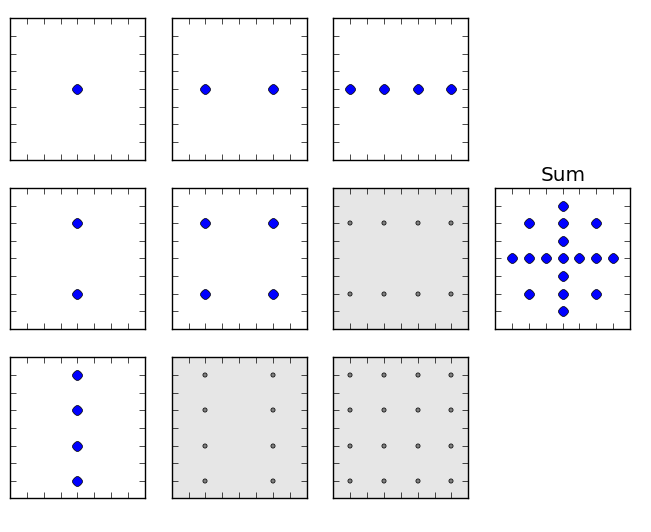
\includegraphics[width=7.5cm]{images/sparsegrid_hirach2}
      \vspace{-12px}
      \caption{}
    \end{figure}
  \end{block}
\end{frame}


\begin{frame}
  \frametitle{Sparse Grids -- Basics}
  \topline
  \vspace{-10px}
  \begin{block}{A sparse grid}
    \begin{table}[h]
      \setbeamertemplate{caption}{\raggedright\insertcaption\par}
      \setbeamerfont{caption}{size=\footnotesize}
      \centering
      \begin{tabular}{r | c | c | c | c | c | c}
        d & 1 & 2 & 3 & 5 & 10 & 20 \\
        \hline\hline
        Full & 15 &  225 & 3375 & $>10^5$ & $> 10^{11}$ & $> 10^{23}$ \\
        \hline
        Sparse & 15 & 49 & 111 & 351 & 2001 & 13201 \\
      \end{tabular}
      \caption{Full grid vs. sparse grid with $n = 4$}
    \end{table}
    \begin{itemize}
    \item Massive difference in high dimensions
    \item Note: No boundary grid points!
    \end{itemize}
  \end{block}
\end{frame}


\begin{frame}
  \frametitle{Sparse Grids -- Basics}
  \topline
  \vspace{-10px}
  \begin{block}{Sparse grid for $n = \{4,5,6,7\}$}
    \begin{figure}[!htp]
      \setbeamertemplate{caption}{\raggedright\insertcaption\par}
      \setbeamerfont{caption}{size=\footnotesize}
      \centering
      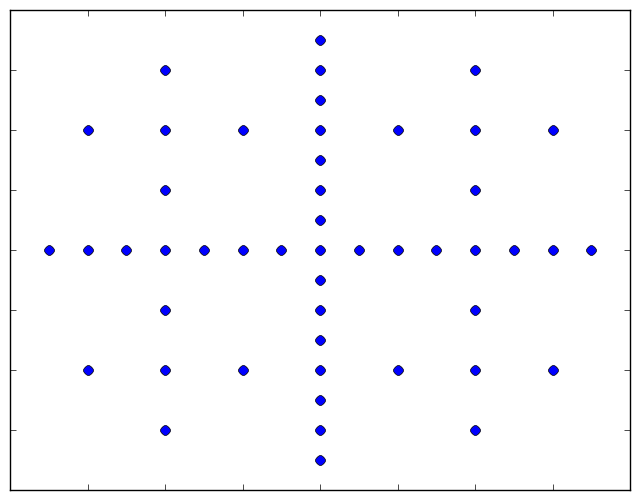
\includegraphics[width=4cm]{images/sparsegrid_d4}
      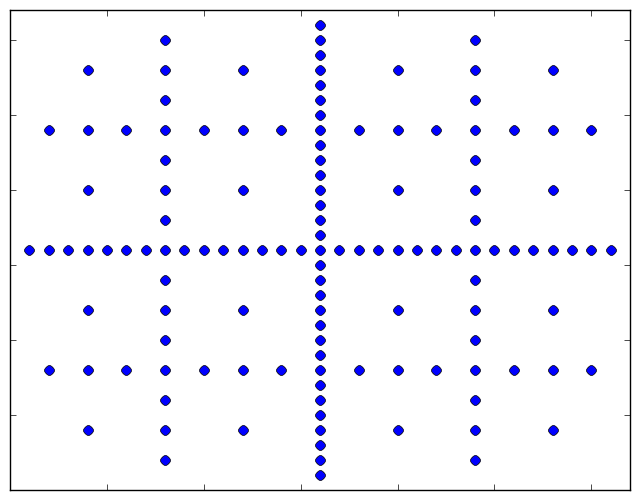
\includegraphics[width=4cm]{images/sparsegrid_d5}
      \\
      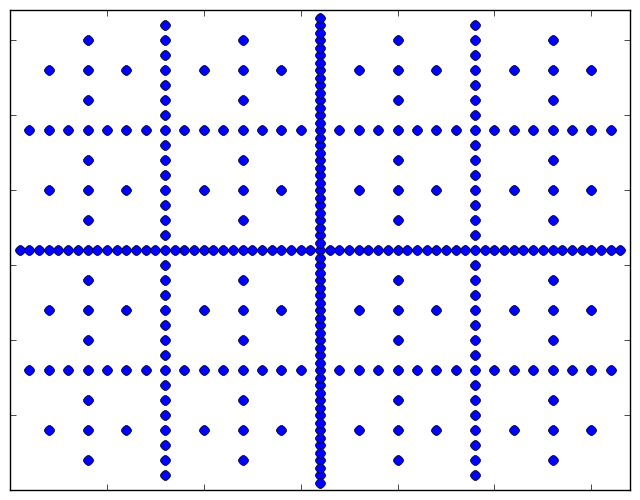
\includegraphics[width=4cm]{images/sparsegrid_d6}
      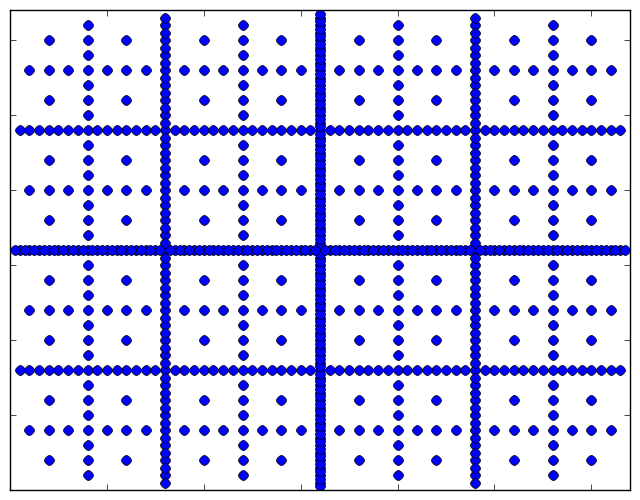
\includegraphics[width=4cm]{images/sparsegrid_d7}
      \vspace{-12px}
      \caption{}
    \end{figure}
  \end{block}
\end{frame}


\begin{frame}
  \frametitle{Sparse Grids -- Basics}
  \topline
  \vspace{-10px}
  \begin{block}{Hierarchical subspaces}
    \begin{figure}[!htp]
      \setbeamertemplate{caption}{\raggedright\insertcaption\par}
      \setbeamerfont{caption}{size=\footnotesize}
      \centering
      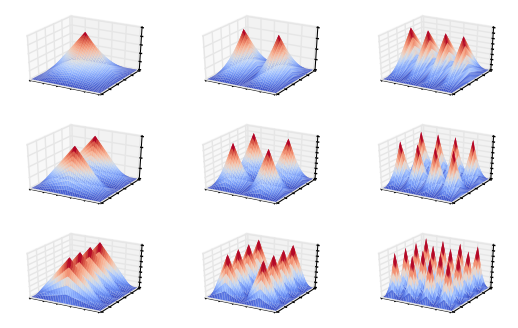
\includegraphics[width=7.5cm]{images/sparsegrid_2dhats}
      \vspace{-12px}
      \caption{}
    \end{figure}
  \end{block}
\end{frame}


\begin{frame}
  \frametitle{Sparse Grids -- Basics}
  \topline
  \vspace{-10px}
  \begin{block}{Adaptivity}
    \begin{figure}[!htp]
      \setbeamertemplate{caption}{\raggedright\insertcaption\par}
      \setbeamerfont{caption}{size=\footnotesize}
      \centering
      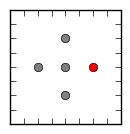
\includegraphics[width=0.2\textwidth]{images/adaptive_0}
      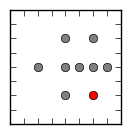
\includegraphics[width=0.2\textwidth]{images/adaptive_1}
      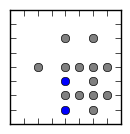
\includegraphics[width=0.2\textwidth]{images/adaptive_2}
      \caption{}
    \end{figure}
    \vspace{-20px}
    \begin{itemize}
      \item \emph{A-posteriori} modifications to model the function better
      \item Adding level of detail around a grid point: $l + 1$
      \item Overfitting possible and considerable computational effort
      \item Multiple strategies possible
      \end{itemize}
  \end{block}
\end{frame}

\begin{frame}
  \frametitle{Sparse Grids -- Basics}
  \topline
  \vspace{-10px}
  \begin{block}{Summary}
    \begin{itemize}
      \item Hierarchical basis through grouping grid points into levels
      \item Creating subspaces through combination of levels in dimensions
      \item Selecting only certain subspaces
      \item Adaptive refinement
      \end{itemize}
      \vspace{20px}
      $$\hat{f}(\vec{x}) = \sum_{l,i}{\alpha_{l,i} \phi_{l,i}(\vec{x})} $$
  \end{block}
\end{frame}

%%% Local Variables:
%%% TeX-master: "slides"
%%% End:
